\part{Attività formative e di ricerca -  \RNum{3} anno}

\section{Corsi e Seminari}
\begin{itemize}
	\item \textbf{UKMAC 2017}, \textit{UK Manycore Developer Conference}, 11 Luglio 2017, University of Warwick
\end{itemize}

\section{Didattica}
\begin{description}
\item [\textbf{Esercitatore}] del corso di\textit{ Interfacce Grafiche e Programmazione ad Eventi} del CdL in \textit{Informatica}, \textit{Dipartimento di Matematica e Informatica}, UNICAL. \textbf{Periodo}: \textit{Marzo 2017 - Settembre 2017}
\end{description}

\section{Visiting presso altre università}
\begin{description}
	\item [da Giugno 2017 a Agosto 2017] presso il \textit{Department of Computer Science, University of Warwick (UK)} sotto la supervisione del Prof. \textit{Gihan R. Mudalige}.
\end{description}


\section{Pubblicazioni}
\begin{itemize}
	\item  Donato D'Ambrosio, Alessio De Rango, Marco Oliverio, Davide Spataro,
	William Spataro, Rocco Rongo, Giuseppe Mendicino, Alfonso Senatore:
	\textbf{The Open Computing Abstraction Layer for Extended Cellular
	Automata and the Finite Di fferences Method}, accepted with revisions to
	the \textit{ISI/SCOPUS Journal of Parallel and Distributed Computing (ISSN:
	0743-7315)}.

\item Donato D'Ambrosio, Alessio De Rango, Davide Spataro, Rocco Rongo,
William Spataro: Applications of the OpenCAL scientific library in
the context of CFD: \textbf{Applications of the \texttt{OpenCAL} scientific library to debris flows}, \textit{2017 IEEE 14th
International Conference on Networking, Sensing and Control (ICNSC)}

\item A. De Rango, D. Spataro, D. D’Ambrosio, R. Rongo, W. Spataro, \textbf{Fast
Lava Risk Assessment by Multi-GPU}, accepted at the \textbf{26th Euromicro
International Conference on Parallel, and Network-Based Computing
2018}, \textit{Cambridge (UK), March 21-23, 2018}

\end{itemize}


\section{Attività di Ricerca}
Durante il mio \RNum{3} anno di dottorato mi sono occupato principalmente di concludere, ottimizzare e testare il lavoro iniziato negli anno precedenti sulla librarie \texttt{OpenCAL}. La librerie si dimostra in grado di produrre implementazioni parallele di una classe di modelli numerici a griglia regolare, utilizzando un formalismo che nasconde sia i dettagli architetturali tecnici dell'hardware sul quale essi sono eseguiti che la complessità intrinseca del parallelismo. La libreria è stata testata su tre modelli differenti per caratteristiche e requirements computazionali. Tre benchmark sono stati adottati:
\begin{enumerate}
	\item Julia Set: \textbf{compute bound}
	\item Convolutional Filter:\textbf{memory/bandiwidth bound}
	\item sciddicaT: \textbf{memory e compute bound}
\end{enumerate} 
La sezione \ref{sec:convolutional_filters} mostra un esempio di implementazione di un semplice filtro convoluzionale (esempiodi memory bound application), \textit{Sobel}, in \texttt{OpenCAL} e i relativi risultati di performance ottenuti.

\subsection{Convolutional Filters}
\label{sec:convolutional_filters}
La convoluzione di un immagine può essere espressa in modo generico mediante la seguente formula:
\begin{equation}
f'_{ij} = \sum_{i'=0}^n (\sum_{j'i'=0}^m f_{(i+i')(j+j')}\times d_{ij})
\label{eq:convolution}
\end{equation}
dover 
\begin{itemize}
	\item $m,n$ sono le dimensioni verticali ed orizzonatali del kernel
	\item $f_{ij}$ e $f'_{ij}$ sono rispettivamente il vecchio ed il nuovo valore della cella alla posizione $(i,j)$,
	\item $d_{ij}$ è il valore del kernel alla posizione $(i,j)$ 
\end{itemize}
\begin{figure}[!htb]
	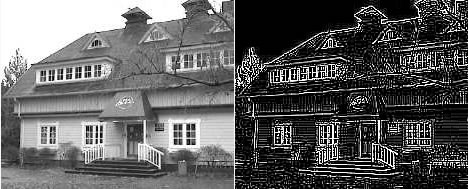
\includegraphics[width=\linewidth]{./images/sobel_example}
	
	\caption{Esempio dell'applicazione del filtro \textit{Sobel} implementato in \texttt{OpenCAL}. }
	\label{fig:sobel}
\end{figure}

Il filtro di Sobel è facilmente implementabile in \texttt{OpenCAL} seguendo gli step che seguono::
\begin{enumerate}
	\item L'immagine viene decomposta nei canali di colore rosso, verde e blu, e ognuno di esso è letto in un sottostato di tipo short.
	\item Un \textit{cluster} file viene definito il quale specifica (si veda Listato \ref{code:sobel_cluster_file}) come il dominio deve essere diviso tra le risorse computazionali a disposizione.
	\item Il codice che implementa l'applicazione di un kernel (si veda Listato \ref{code:sobel_kernel}) a un signolo punto del dominio viene specificato dal programmatore e automaticamente eseguito in parallelo su tutto il dominio. Se un device necessita di dati che sono stati assegnati ad un altro device, questi vengono automaticamente trasferiti in maniera trasparente, anche quando essi sono fisicamente installati su nodi separati (in quel caso attraverso anche una comunicazione MPI).
\end{enumerate}
\begin{figure}
	\centering
	\caption{Sobel Scaling}
	\label{fig:sobel_scaling}
	\includegraphics[width=0.6\textwidth]{../plots/sobel_scaling}
\end{figure}
\lstset{language=[OpenCL]C,frame=tb,
	caption=Adopted cluster file for the Sobel filtering example. The image is decomposed equally among 3 devices. , 
	basicstyle=\footnotesize\ttfamily,
	label={code:sobel_cluster_file}
}
\begin{lstlisting}[float]
10800 21600
1
192.168.1.111 3
0 0 3600
0 1 3600
0 2 3600
\end{lstlisting}
Figure \ref{fig:sobel_scaling} mostra come il filtro Sobel scala al crescere del numero delle GPU utilizzate. Si noti come schede diversi tipi di schede (marca ed architettura) possono essere utilizzate allo stesso momento.
La  Figura \ref{fig:sobel_2nodes_performance} mostra lo stesso codice eseguito su due nodi differenti. Come si può vedere anche in questo caso, in cui una comunicazione via rete è necessaria, buone performance sono ottenute, con un picco di $\approx 81\times$ quando tre devices sono utilizzati in modo concorrente.
La libreria supporta anche architetture distributed memory e,la Figura \ref{fig:sobel_2nodes_k40+980-K20+980} mostra tempi e speedups per un esecuzione su due nodi, ognuno dei quali equipaggiato con due acceleratori (per un totale di $4$). 
In questo caso è stato ottenuto un miglioramento di circa $\apoprox 22 \times$ e $\approx 103$ rispetto ad un esecuzione su $3$ GPU su un singolo nodo (si veda Figura \ref{fig:sobel_scaling}) e l'esecuzione \textbf{seriale} su un singolo core.
\begin{figure}[!htb]
	\minipage{1.0\textwidth}
	\begin{subfigure}{1.0\textwidth}
		\caption{Performance on $2$ nodes and $2$ GPUs: \texttt{NVIDIA K40}(\textit{node 1}) and $1$ \texttt{GTX980}(\textit{node 2}).}
		\label{fig:sobel_2nodes_k40_980}
		\includegraphics[width=1.0\textwidth]{../plots/sobel_2nodes_k40_980}
		
	\end{subfigure}        
	\endminipage \hfill
	\minipage{1.0\textwidth}
	\vspace{5mm}
	\begin{subfigure}{1.0\textwidth}
		\includegraphics[width=1.0\textwidth]{../plots/sobel_2nodes_k40+980-K20+980}
		\caption{Performance on $2$ nodes each with $2$ GPUs.}
		\label{fig:sobel_2nodes_k40+980-K20+980}
	\end{subfigure}
	\endminipage\hfill
	\caption[\textit{Sobel} filter benchmark performance metrics on two nodes.]{\textit{Sobel} filter benchmark performance metrics on two Ethernet interconnected nodes. (a) reefers to the case where node 1 is equipped with $1$ $K40$ and node 2 with a $GTX980$. (b) to the case where \textit{node 1} uses a $K40$ and a $GTX980$ while \textit{node 2} a $K20$ and a $GTX980$. Time in red (lower is better), speed-up in blue (higher is better).}
	\label{fig:sobel_2nodes_performance}
\end{figure}
\begin{minipage}{1.0\textwidth}


\lstset{language=[OpenCL]C,frame=tb,
	caption=\texttt{OpenCAL} Sobel edge detection filter kernel., 
	label={code:sobel_kernel}, 
	basicstyle=\footnotesize\ttfamily,
	keywordstyle=\color{blue}\ttfamily,
	stringstyle=\color{red}\ttfamily,
	commentstyle=\color{green}\ttfamily,
	backgroundcolor=\color{light-gray}, 
	numbers=left,numbersep=3pt, 
	numberstyle=\tiny\ttfamily\color{gray}
	%    numberstyle=\tiny
}
\begin{lstlisting}
__kernel void sobel2D_transitionFunction(__CALCL_MODEL_2D) {
	calclThreadCheck2D();
	int i = calclGlobalRow() + borderSize;
	int j = calclGlobalColumn();
	int KX[3][3] = {{-1, 0, 1}, {-2, 0, 2}, {-1, 0, 1}};
	int KY[3][3] = {{1, 2, 1}, {0, 0, 0}, {-1, -2, -1}};
	int Gx, Gy, n, k, k1;
	Gx = Gy = n = 0;
	if (j > 0 && j < calclGetColumns() - 1)
		for (k = -1; k <= 1; k++)
			for (k1 = -1; k1 <= 1; k1++) {
				Gx += calclGet2Di(MODEL_2D, DEVICE_Q_red, i + k, j + k1) *
				KX[k + 1][k1 + 1];
				Gy += calclGet2Di(MODEL_2D, DEVICE_Q_red, i + k, j + k1) *
				KY[k + 1][k1 + 1];
			}
	const int P = sqrt(Gx * Gx + Gy * Gy);
	// set new pixel color for red channel
	calclSet2Di(MODEL_2D, DEVICE_Q_red, i, j, P);
	return;
}
\end{lstlisting}
\end{minipage}